\section{债券模型和利率衍生品定价}
\begin{enumerate}
    \item 假设10000元用于2年期的投资,以下四种投资方案哪种收益最佳?
    \begin{enumerate}[label=\Alph*.]
        \item 简单复利年利率为9.5\%。
        \item 年利率为9\%,第一年每月复利一次,第二年每半年复利一次。
        \item 年利率为9.2\%,第一年每三个月复利一次,第二年每月复利一次。
        \item 连续复利年利率为9\%。
    \end{enumerate}
    \sol
    \begin{enumerate}[label=\Alph*.]
        \item $10000 \times (1+9.5\%)^2 = 11990.25.$
        \item $\displaystyle 10000 \times \left(1 + \frac{9\%}{12}\right)^{12} \times \left(1 + \frac{9\%}{2}\right)^2 = 11944.64.$
        \item $\displaystyle 10000 \times \left(1 + \frac{9.2\%}{4}\right)^{4} \times \left(1 + \frac{9.2\%}{12}\right)^{12} = 12003.43.$
        \item $10000 \times \left(\mathrm{e}^{9\%}\right)^2 = 11972.17.$
    \end{enumerate}
    故投资方案C收益最佳。
    \item 假设到期日为$T$的零息债券在$t(t \leqslant T)$时刻的价格为
    \[B(t,T)=\frac{1}{(1+r)^{T-t}}, \quad r>-1\]
    分别计算简单复利和连续复利下的即息利率和远期利率。\\
    \sol\\
    简单复利的即息利率:
    \[L(t, T) = -\frac{B(t,T) - 1}{(T - t)B(t, T)} = -\frac{\left({\left(1 + r\right)}^{t - T} - 1\right) {\left(1 + r\right)}^{T - t}}{T - t}.\]
    连续复利的即息利率:
    \[R(t, T) = -\frac{\ln B(t, T)}{T - t} = \ln (1 + r).\]
    简单复利的远期利率:
    \[L(t, S, T) = -\frac{B(t,T)-B(t,S)}{(T-S)B(t,T)}=\frac{{\left(1 + r\right)}^S - {\left(1 + r\right)}^T}{\left(S - T\right) {\left(1 + r\right)}^S}.\]
    连续复利的远期利率:
    \[R(t,S,T) = -\frac{\ln B(t,T) - \ln B(t,S)}{T-S} = \ln (1 + r).\]
    \item 假设到期日为$T$的零息债券在$t(t \leqslant T)$时刻的价格为
    \[B(t,T)=\mathrm{e}^{-r(T-t)}\]
    分别计算简单复利和连续复利下的即息利率和远期利率。\\
    \sol\\
    简单复利的即息利率:
    \[L(t, T) = -\frac{B(t,T) - 1}{(T - t)B(t, T)} = -\frac{\mathrm{e}^{r \left(T - t\right)} \left(\mathrm{e}^{- r \left(T - t\right)} - 1\right)}{T - t}.\]
    连续复利的即息利率:
    \[R(t, T) = -\frac{\ln B(t, T)}{T - t} = r.\]
    简单复利的远期利率:
    \[L(t, S, T) = -\frac{B(t,T)-B(t,S)}{(T-S)B(t,T)}=\frac{\mathrm{e}^{r \left(T - S\right)} - 1}{T - S}.\]
    连续复利的远期利率:
    \[R(t,S,T) = -\frac{\ln B(t,T) - \ln B(t,S)}{T-S} = r.\]
    \item 对于下图给出的时间4到期的零息债券价格树,请计算出其余不同到期日的债券价格和短期利率,画出债券价格期限结构二叉树模型。\textcolor{red}{(补充:时间步长$\displaystyle\delta = \frac{1}{12}$,下图中的$B(0,3)=0.9927$)}
    \begin{center}
        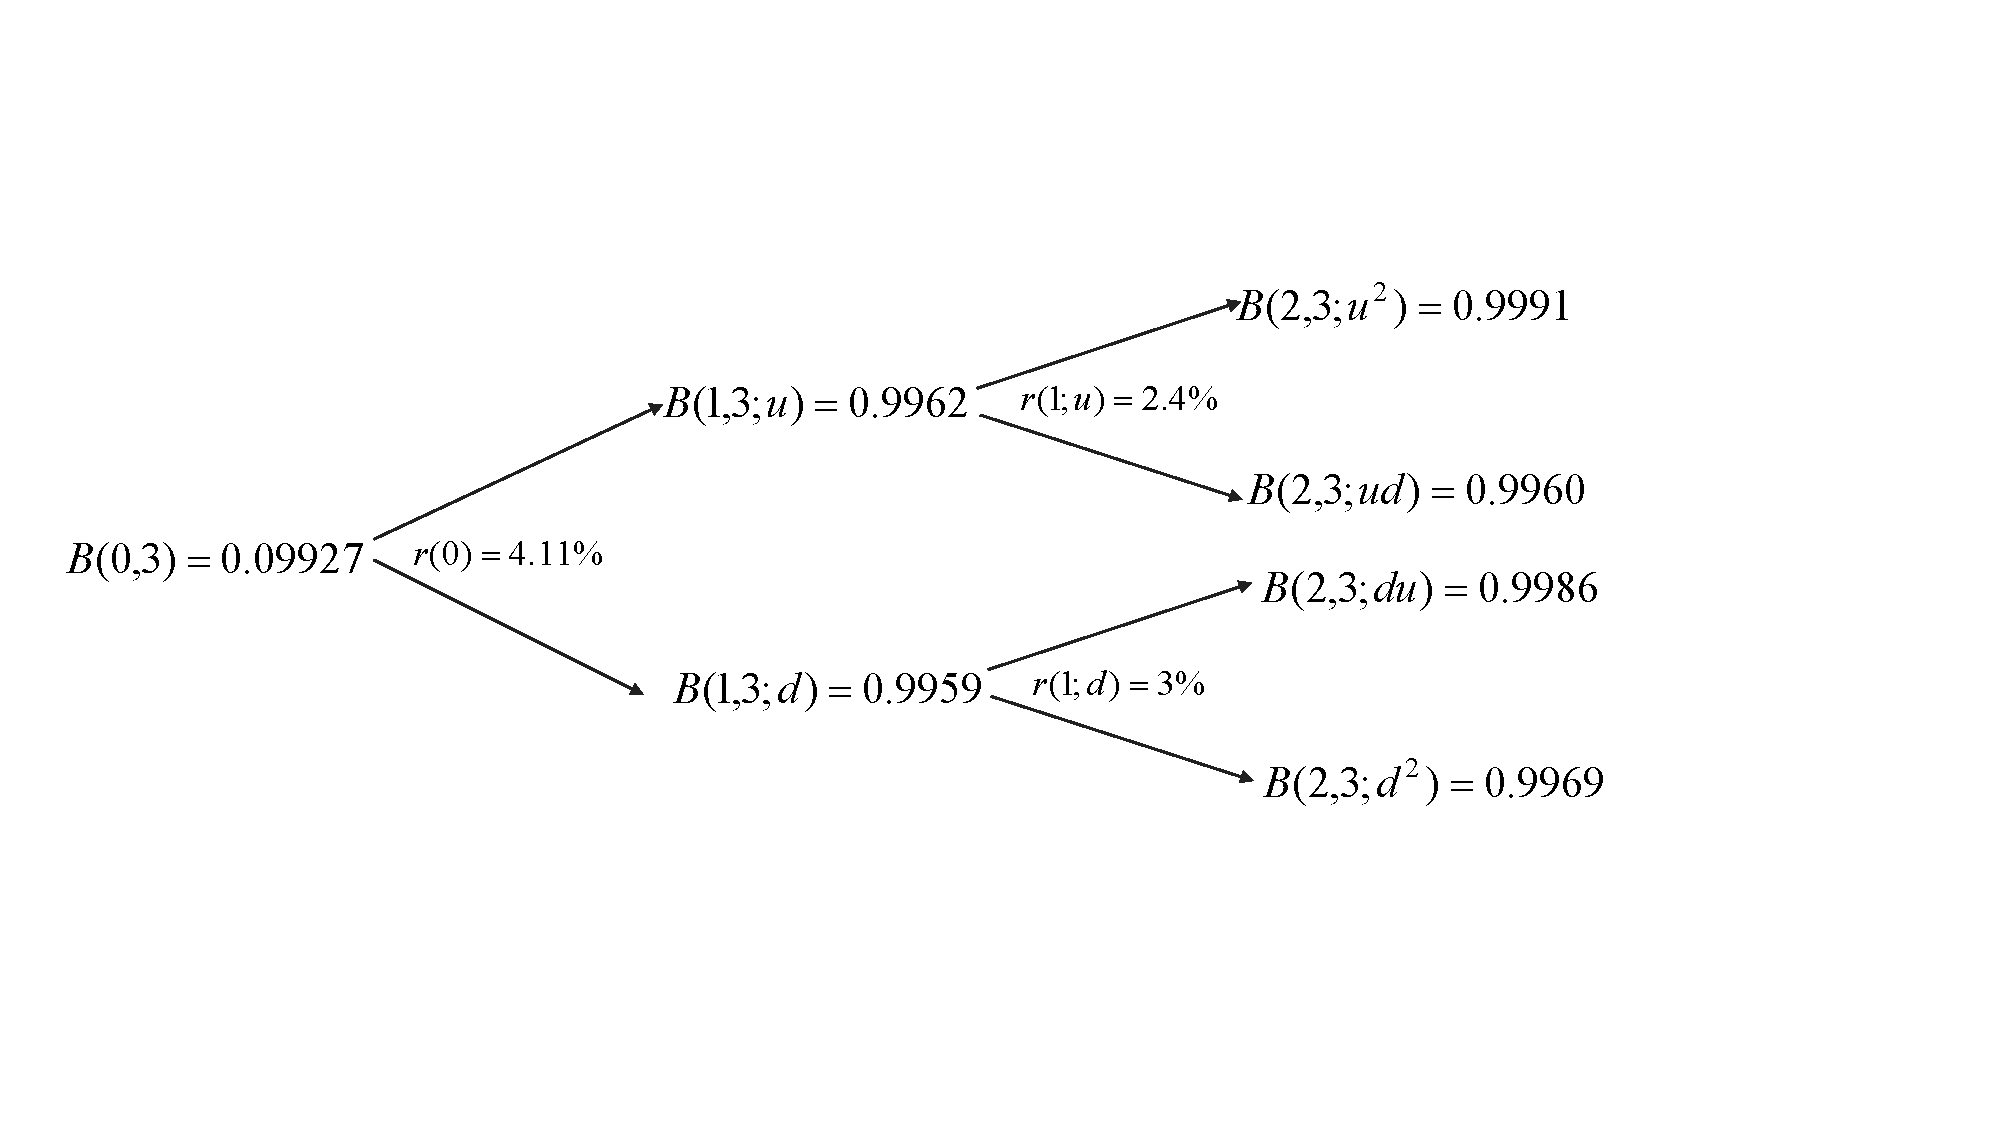
\includegraphics[scale=0.5]{8-4.pdf}
    \end{center}
    \sol\\
    短期利率读图便可知:
    \[r(0)=4.11\%,r(1;u)=2.4\%,r(1;d)=3\%.\]
    为计算债券价格,首先我们可以计算出二叉树上每一步的风险中性概率
    \begin{align*}
        p(0) & = \frac{B(0,3)[1+\delta r(0)]-B(1,3;d)}{B(1,3;u)-B(1,3;d)} = 0.6667,\\
        p(1;u) & = \frac{B(1,3;u)[1+\delta r(1;u)]-B(2,3;ud)}{B(2,3;u^2)-B(2,3;ud)} = 0.7072,\\
        p(1;d) & = \frac{B(1,3;d)[1+\delta r(1;d)]-B(2,3;d^2)}{B(2,3;du)-B(2,3;d^2)} = 0.8763.
    \end{align*}
    对于不同到期日的债券价格,我们以倒推的形式从二叉树末尾往前推到树的起点。因为$B(2,2)=1$,利用式(8-13)可得
    \begin{align*}
        B(1,2;u) & = \frac{1}{1 + \delta r(1;u)}[p(1;u)B(2,2)+[1-p(1;u)]B(2,2)] = 0.9980,\\
        B(1,2;d) & = \frac{1}{1 + \delta r(1;d)}[p(1;d)B(2,2)+[1-p(1;d)]B(2,2)] = 0.9975.
    \end{align*}
    接着再利用式(8-13)从后往前计算
    \[B(0,2)=\frac{1}{1 + \delta r(0)}[p(0)B(1,2;u)+(1-p(0))B(1,2;d)]=0.9944,\]
    同样地因为$B(1,1)=1$,因此利用式(8-13)可得
    \[B(0,1)=\frac{1}{1 + \delta r(0)}[p(0)B(1,1)+(1-p(0))B(1,1)]=0.9966.\]
    最后我们可以得到如下图所示的债券价格期限结构二叉树:
    \begin{center}
        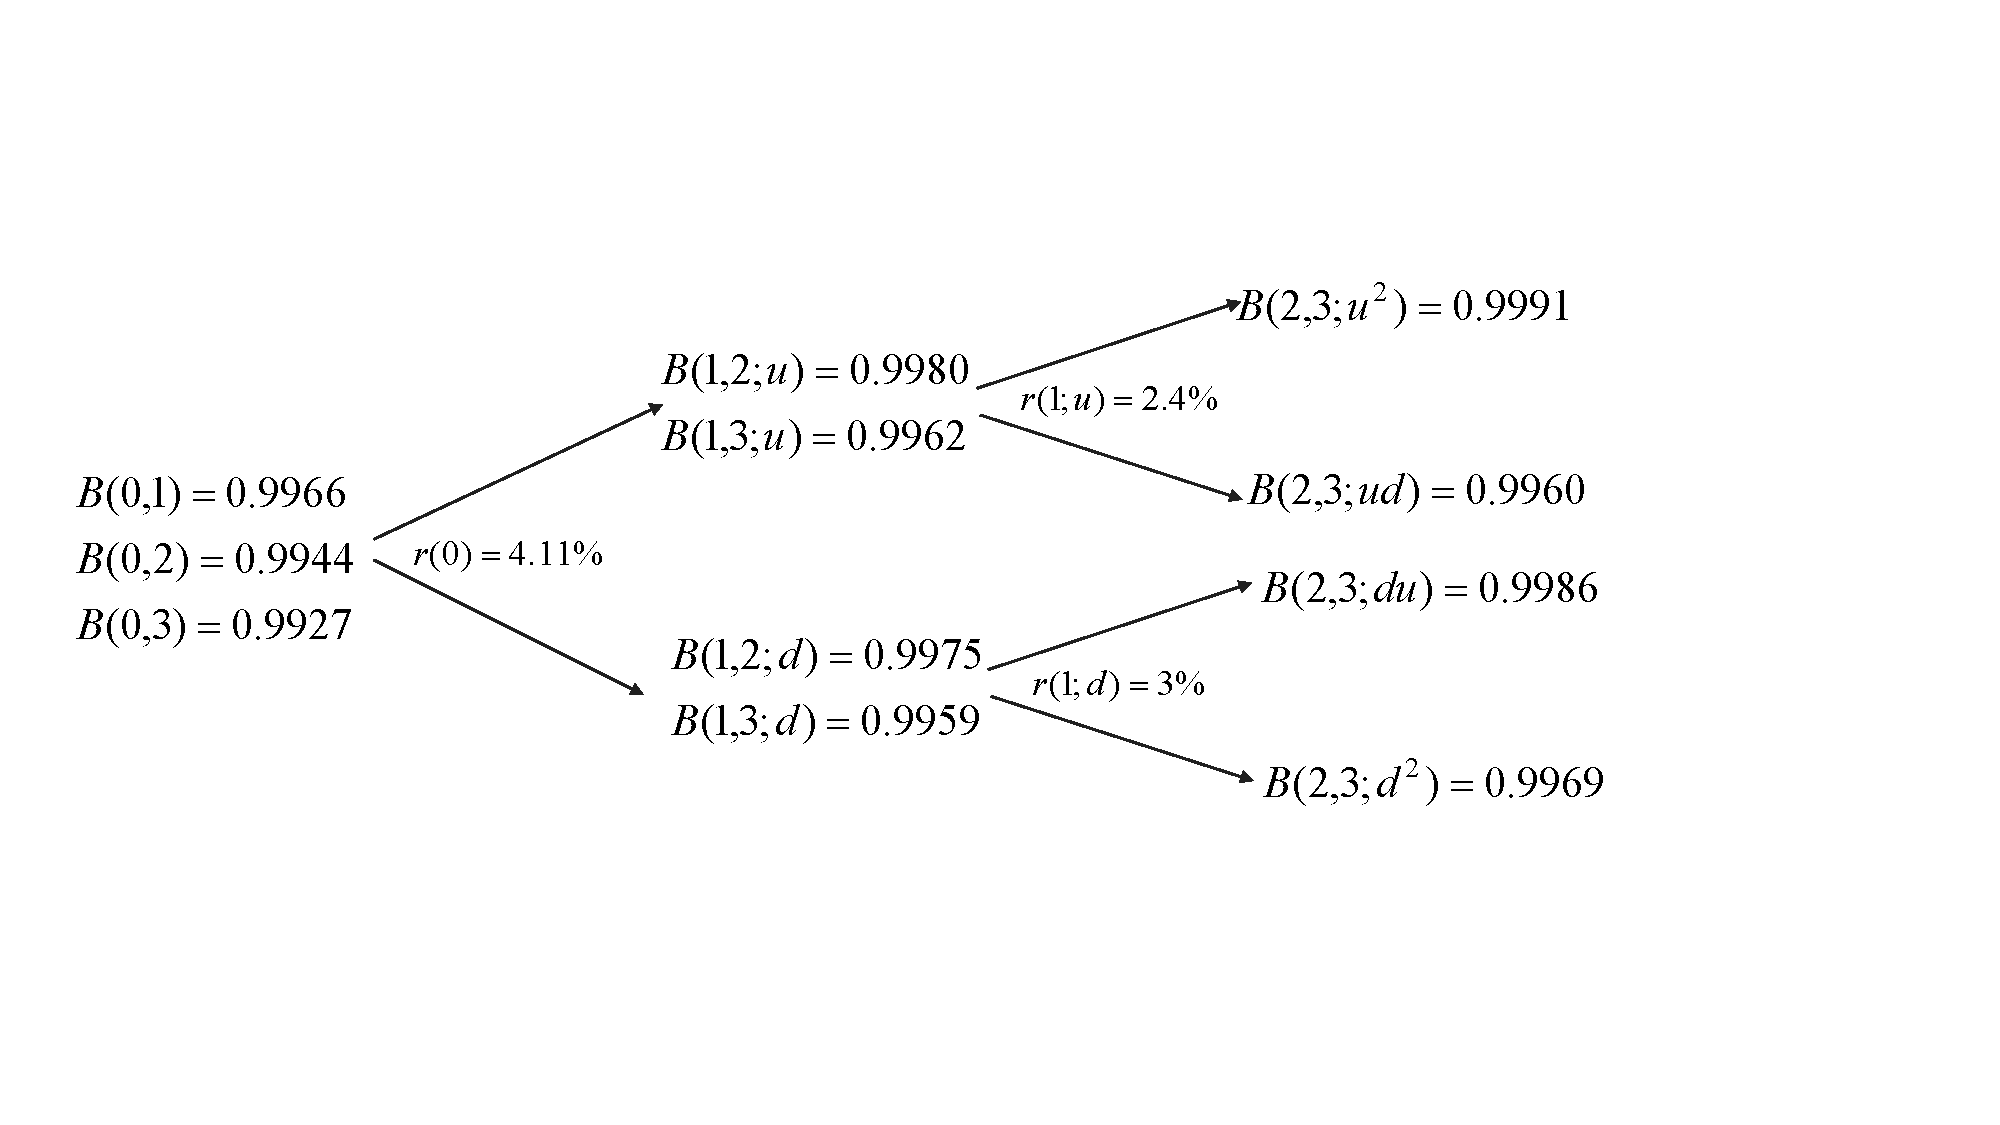
\includegraphics[scale=0.5]{8-4-sol.pdf}
    \end{center}
    \item 利用上题中的期权价格,计算在时间3到期的零息债券看涨期权,该期权的施权日2,施权价为0.9965。求该期权的价格。\\
    \sol\\
    首先我们根据上图最后1列债券的价格计算出期权的最终收益,再利用风险中性概率和短期利率进行贴现,同时结合式(7-9)和式(7-10),从树的末端往前倒推最终计算出期权的价格,见下图。
    \begin{center}
        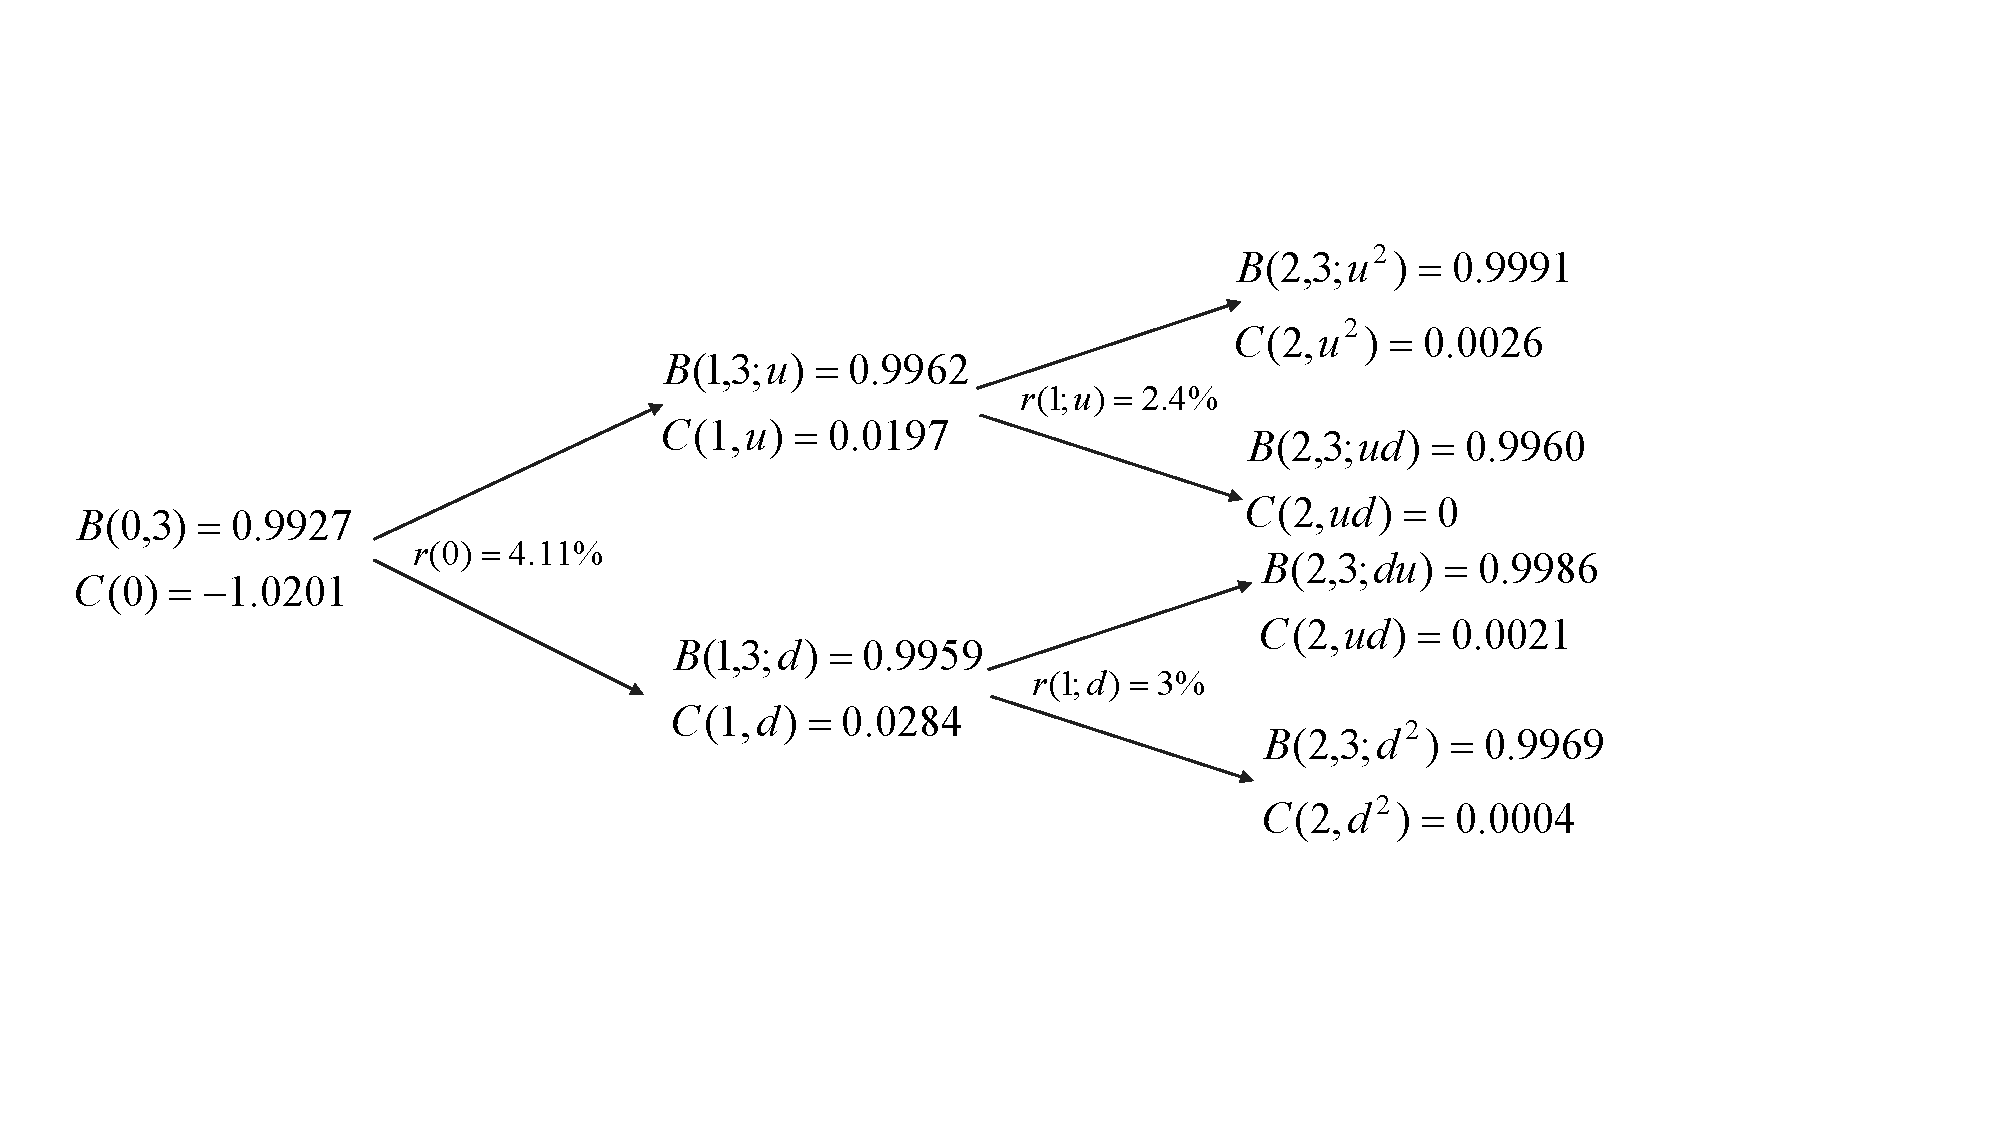
\includegraphics[scale=0.5]{8-5.pdf}
    \end{center}
    \item 假设$t<S<T$。请利用简单复利即息利率$L(t,S)$和$L(t,T)$给出简单复利远期利率$L(t,S,T)$的表达式;利用连续复利即息利率$R(t,S)$和$R(t,T)$给出连续复利远期利率$R(t,S,T)$的表达式。假设$L(0,1/2)=7\%,L(0,1)=6\%$,请计算远期利率$L(0,1/2,1)$和$R(0,1/2,1)$。\\
    \sol\\
    因为$\displaystyle L(t, T) = -\frac{B(t,T) - 1}{(T - t)B(t, T)}$,所以$\displaystyle B(t, T) = \frac{1}{1 + L(t, T)(T - t)}, B(t, S) = \frac{1}{1 + L(t, S)(S - t)}$,则
    \begin{align*}
        L(t,S,T) & = -\frac{B(t,T)-B(t,S)}{(T-S)B(t,T)} = -\frac{\frac{1}{1 + L(t, T)(T - t)} - \frac{1}{1 + L(t, S)(S - t)}}{(T-S)\frac{1}{1 + L(t, T)(T - t)}} \\
        & = - \frac{1 - \frac{1 + L(t, T)(T - t)}{1 + L(t, S)(S - t)}}{T-S} = \frac{L(t, T)(T - t) - L(t, S)(S - t)}{(T-S)[1 + L(t, S)(S - t)]}
    \end{align*}
    故$\displaystyle L(t,S,T) = \frac{L(t, T)(T - t) - L(t, S)(S - t)}{(T-S)[1 + L(t, S)(S - t)]}$。\\
    因为$\displaystyle R(t, T) = -\frac{\ln B(t, T)}{T - t}$,所以$\displaystyle B(t, T) = \frac{1}{\exp\left[R(t, T)(T - t)\right]}, B(t, S) = \frac{1}{\exp\left[R(t, S)(S - t)\right]}$,则
    \begin{align*}
        R(t, S, T) & = -\frac{\ln B(t,T) - \ln B(t,S)}{T-S} = -\frac{\ln \frac{1}{\exp\left[R(t, T)(T - t)\right]} - \ln \frac{1}{\exp\left[R(t, S)(S - t)\right]}}{T-S}\\
        & = -\frac{R(t, S)(S - t) - R(t, T)(T - t)}{T-S} = \frac{R(t, T)(T - t) - R(t, S)(S - t)}{T-S}
    \end{align*}
    故$\displaystyle R(t, S, T) = \frac{R(t, T)(T - t) - R(t, S)(S - t)}{T-S}$。\\
    因为$L(0,1/2)=7\%,L(0,1)=6\%$,所以
    \[L(0,1/2,1) = \frac{L(0, 1)(1 - 0) - L(0, 1/2)(1/2 - 0)}{(1-1/2)[1 + L(0, 1/2)(1/2 - 0)]} = 4.83\%,\]
    故$L(0,1/2,1) = 4.83\%$。\\
    因为$L(0,1/2)=7\%,L(0,1)=6\%$,所以$\displaystyle B(0,1/2) = \frac{200}{207}, B(0, 1) = \frac{50}{53}$,所以
    \[R(0, 1/2, 1) = -\frac{\ln B(0,1) - \ln B(0,1/2)}{1-1/2} = 4.77\%,\]
    故$R(0,1/2,1) = 4.77\%$。
    \item 给定如下零息债券价格树模型,考虑是否会出现套利机会?若有,请构造一个套利策略。
    \begin{center}
        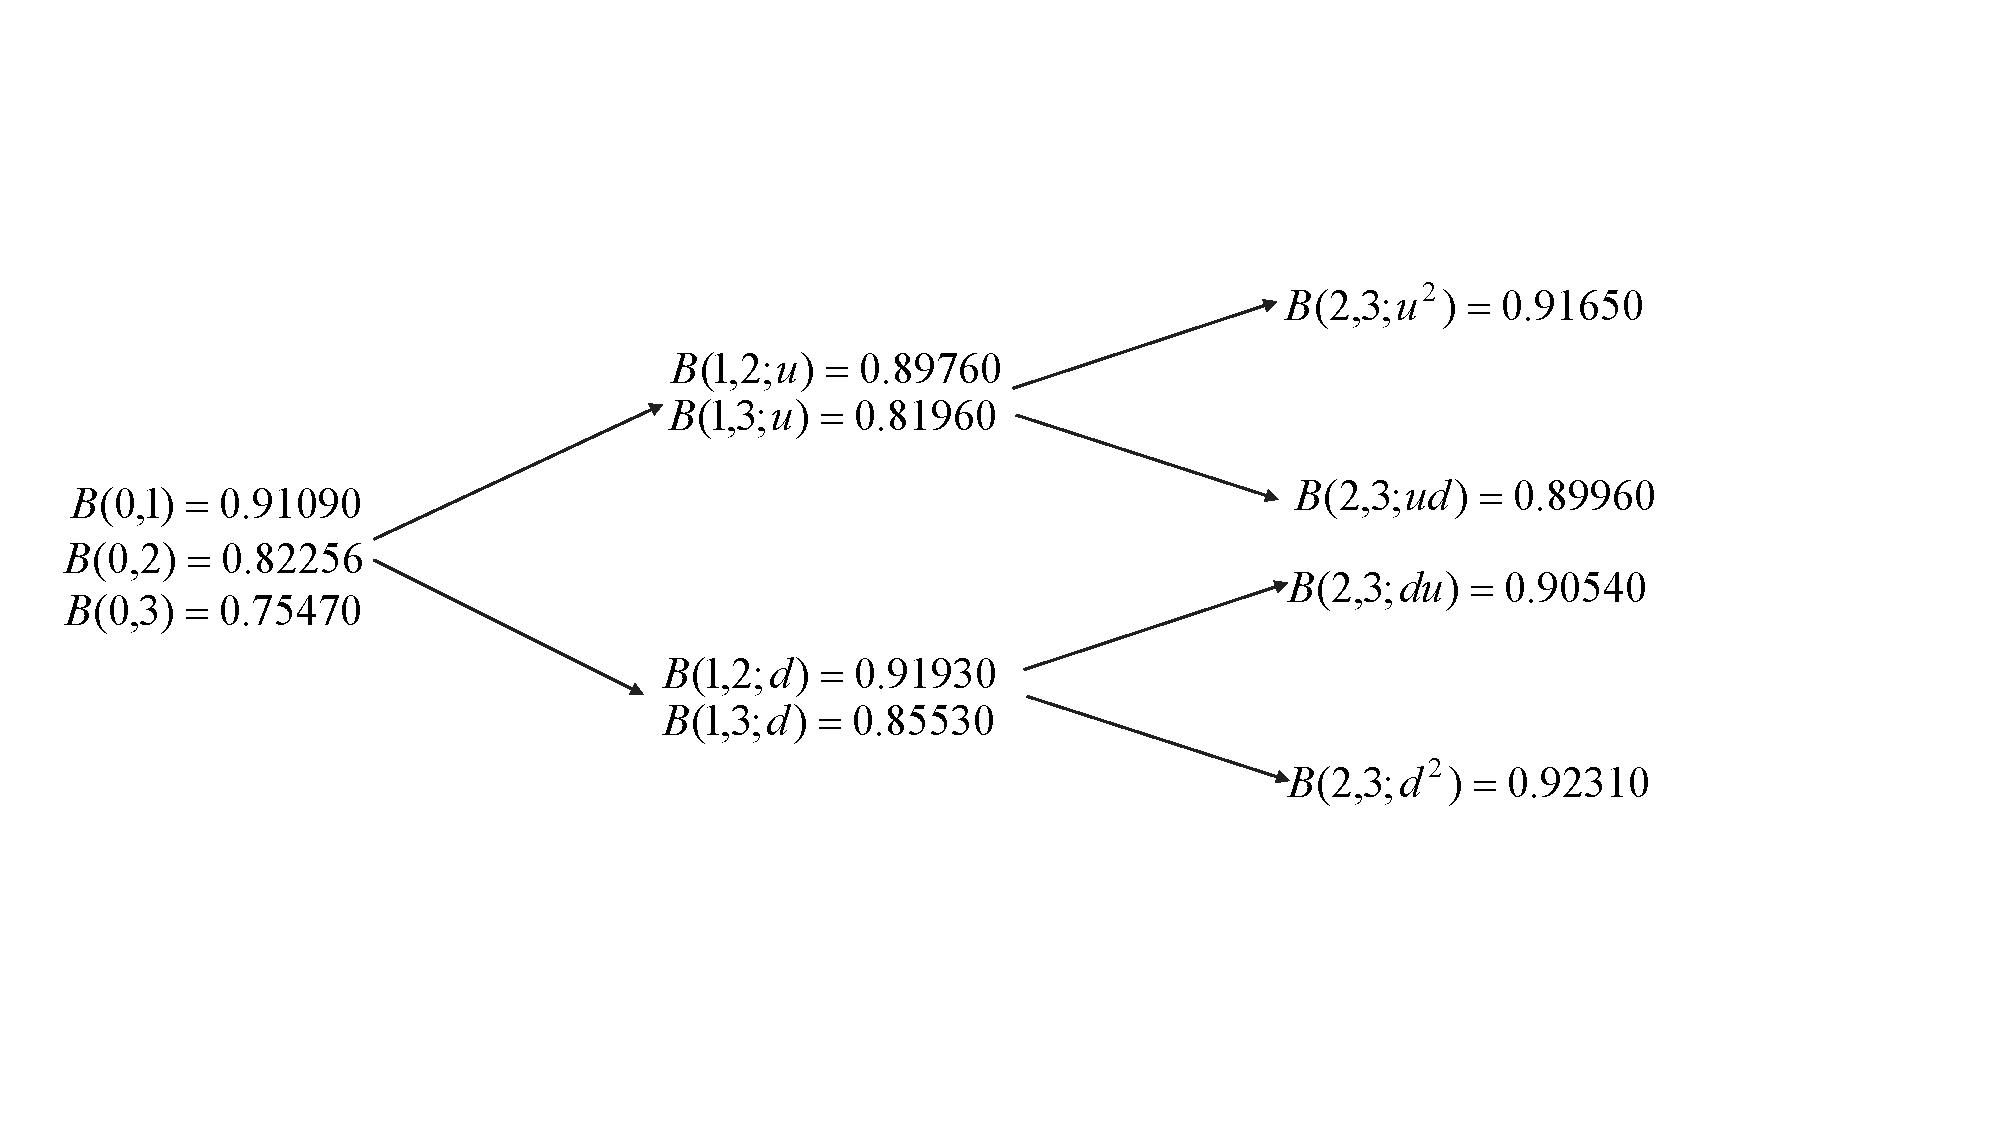
\includegraphics[scale=0.5]{8-7.pdf}
    \end{center}
    \sol\\
    计算风险中性概率:
    \begin{align*}
        p(0, 2) & = \frac{B(0,2)-B(0,1)B(1,2;d)}{B(0,1)B(1,2;u)-B(0,1)B(1,2;d)} \approx 0.75 \in (0,1),\\
        p(0, 3) & = \frac{B(0,3)-B(0,1)B(1,3;d)}{B(0,1)B(1,3;u)-B(0,1)B(1,3;d)} \approx 0.75 \in (0,1),\\
        p(1,3;u) & = \frac{B(1,3;u)-B(1,2;u)B(2,3;ud)}{B(1,2;u)B(2,3;u^2)-B(1,2;u)B(2,3;ud)} \approx 0.7989 \in (0,1),\\
        p(1,3;d) & = \frac{B(1,3;d)-B(1,2;d)B(2,3;d^2)}{B(1,2;d)B(2,3;du)-B(1,2;d)B(2,3;d^2)} \approx -0.4114 \notin (0,1)
    \end{align*}
    故该债权价格二叉树模型不存在套利机会。% 构造套利策略略。
    % \\建立一个资产组合$(x,y)$,这里$x$是时间2到期的债券数,$y$是时间1到期的债券数,使得这个资产组合在时间1的价值等于时间3到期的债券在时间1的价格,即
    % \[\begin{cases}
    %     xB(1,2;u) + yB(1,1) = B(1,3;u)\\
    %     xB(1,2;d) + yB(1,1) = B(1,3;d)
    % \end{cases}\]
    % 可以求得$x = 1.64516, y = -0.65710$。由此我们可以设计以下套利机会:\\
    % 在时间0,卖空65.710份时间1到期的面值为100美元的零息债券,卖空100份时间2到期的面值为100美元的债券,买入164.516份时间2到期的面值为100美元的零息债券,那么还剩余资金
    % \[65.710 \times 100 \times B(0,1) + 100 \times 100 \times B(0,3) - 164.516 \times 100 \times B(0,2) = 1115.59\,(\text{美元}),\]
    % 在时间1,结清所有的债券,即买入164.516份时间1到期的面值为100美元的零息债券,买入100份时间3到期的面值为100美元的债券,同时65.710份时间2到期的面值为100美元的零息债券到期。\\
    % 在节点$u$,收益为
    % \[-164.516 \times 100 \times B(1,1) - 100 \times 100 \times B(1,3;u) + 65.710 \times 100 \times B(1,2;u) = -18749.47\,(\text{美元}),\]
    % 在节点$d$,收益为
    % \[-164.516 \times 100 \times B(1,1) - 100 \times 100 \times B(1,3;d) + 65.710 \times 100 \times B(1,2;d) = -0.04\,(\text{美元}),\]
    \item 利用下图的债券价格二叉树,计算时间2施权,施权利率为3\%的利率下限在时间0的价格。
    \begin{center}
        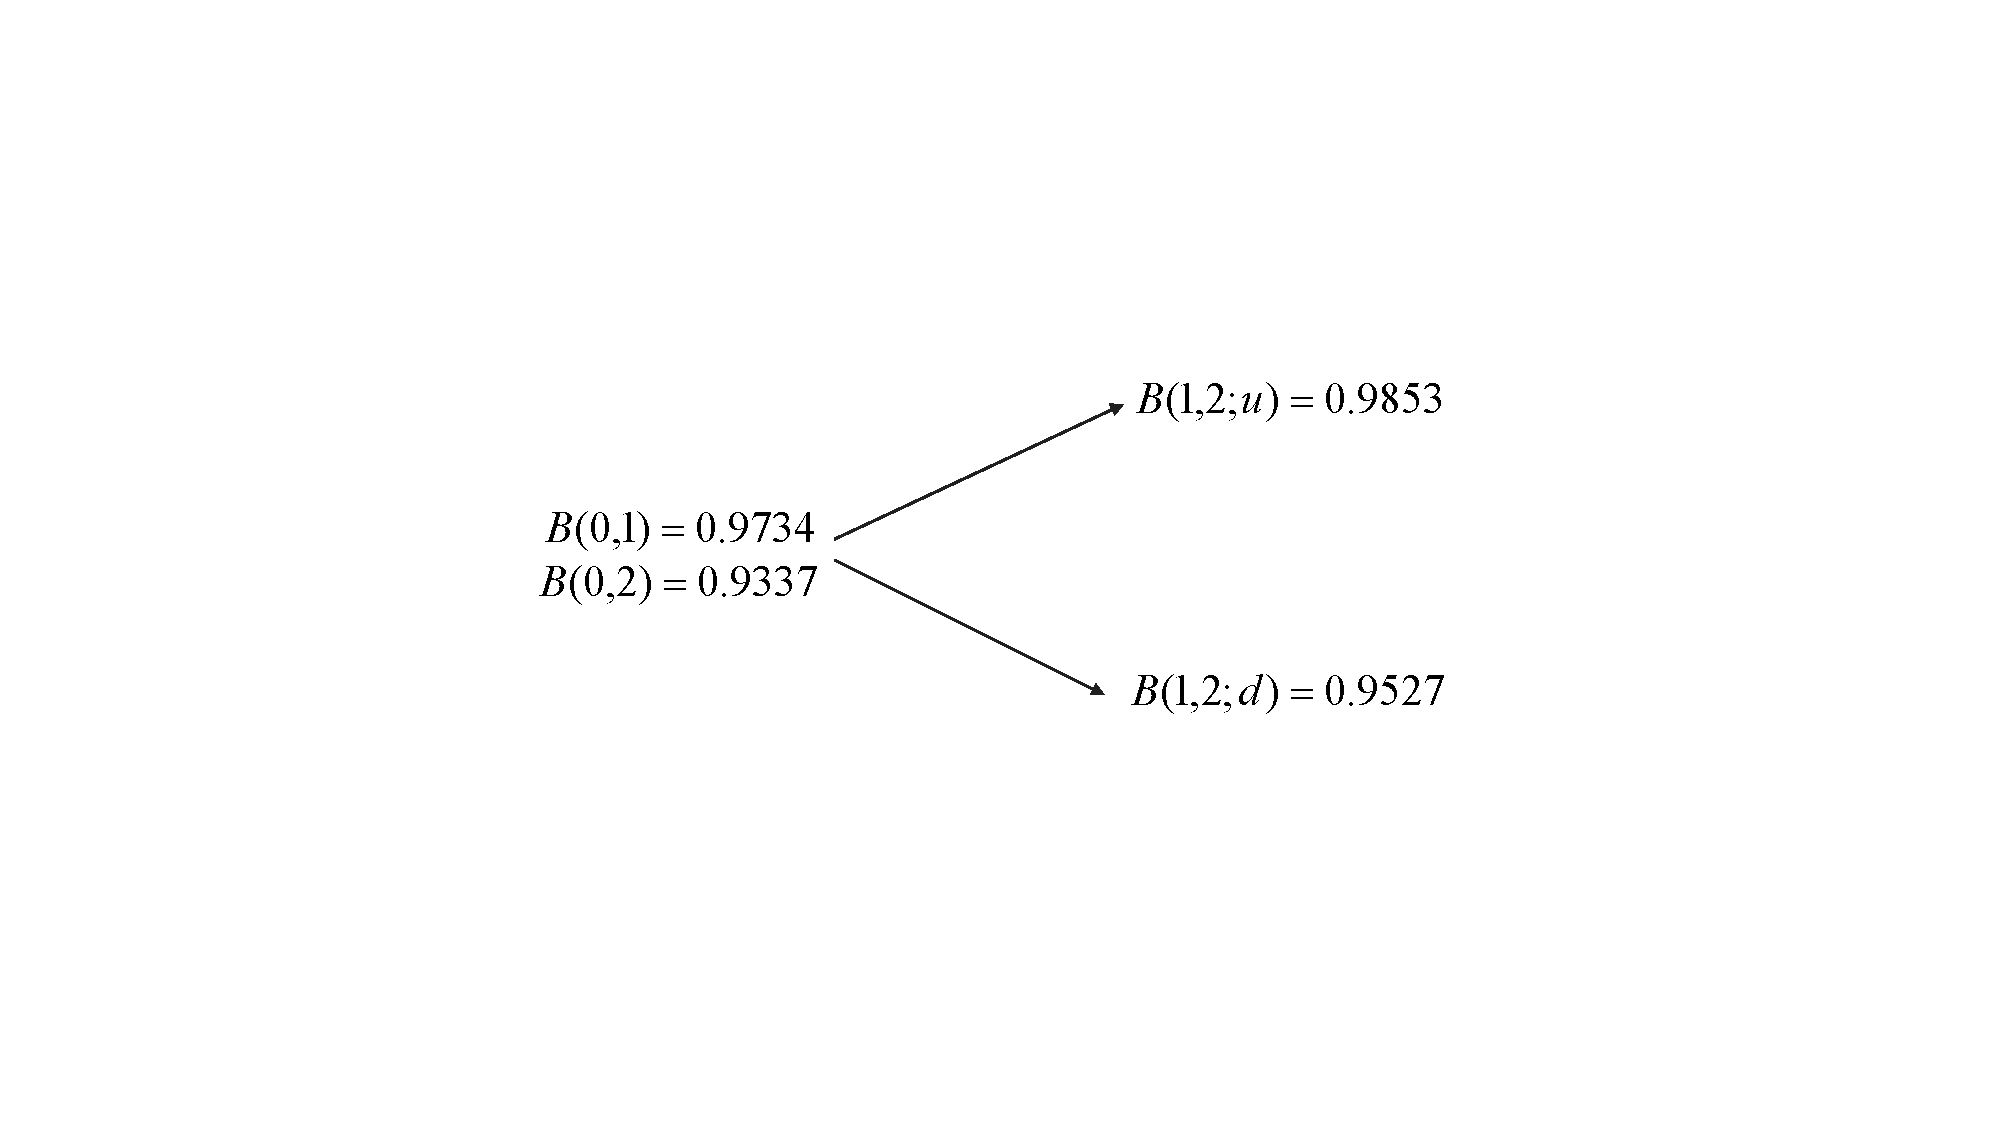
\includegraphics[scale=0.5]{8-8.pdf}
    \end{center}
    \sol\\
    由题知:$F=100,\delta=1,K=0.03,j=0$,则
    \[\frac{F(1+\delta K)}{B(j,j+1)}\max\left\{B(j,j+1)-\frac{1}{1+\delta K},0\right\}=0.2673.\]
    故价格为0.2673。
\end{enumerate}
\clearpage